\documentclass{article}

% The file ijcai16.sty is the style file for IJCAI-16 (same as ijcai07.sty).
\usepackage{ijcai16}

% Packages
\usepackage{./std_package_reqs}

% Definitions
\usepackage{./definitions}

\usepackage{verbatim}

% Graphics Path
\graphicspath{{./images/}}

\renewcommand*{\mkbibparens}[1]{{\ifcitation{\bibleftbracket#1\bibrightbracket}%
        {\bibleftparen#1\bibrightparen}}}
\renewcommand*{\bibopenparen}[1]{{\ifcitation{\bibleftbracket#1}{\bibleftparen#1}}}
\renewcommand*{\bibcloseparen}{{\ifcitation{\bibrightbracket}{\bibrightparen}}}

% Bibliography
\addbibresource{references.bib}

\begin{document}
    
%--------------------------------------------------------------------------------------------------
% Front Matter
%--------------------------------------------------------------------------------------------------

    \title{Analytic Decision Analysis via Symbolic Dynamic Programming for Parameterized Hybrid MDPs}

%\author{Shamin Kinathil \\
%ANU and Data61, CSIRO \\
%Canberra, ACT, Australia \\
%shamin.kinathil@anu.edu.au \\
%\And
%Harold Soh \\
%University of Toronto \\
%Toronto, Ontario, Canada \\
%harold.soh@utoronto.ca \\
%\And
%Scott Sanner  \\
%University of Toronto \\
%Toronto, Ontario, Canada \\
%ssanner@mie.utoronto.ca \\
%}

\maketitle
    \begin{abstract}

Markov Decision Processes (MDPs) provide a powerful framework for
decision-theoretic planning.  While MDPs occur in many applications,
their applicability is limited by the common assumption that the model
parameters are known.  However, there are many settings where it is
important to solve or evaluate MDPs in the presence of uncertainty
over parameters, for example: (i) to investigate the trade-off between
different reward criteria in a multi-objective setting; (ii) to
perform sensitivity analyses of policies to various parameter
settings; and (iii) to analyse and optimise policy performance as a
function of policy parameters. However, formalizing MDPs in this way
leads to a family of hybrid (mixed discrete and continuous state and
action) MDPs with non-linear and/or piecewise structure. In this paper
we show how each of the aforementioned use cases can be formalized
under the common framework of parameterized hybrid MDPs and solved
exactly and in closed-form by leveraging techniques from symbolic
dynamic programming. Our novel framework allows one to explore for the
first-time: (i) an exact functional representation of the
multi-objective trade-offs for use in (Interactive) Decision Maps;
(ii) exact sensitivity analysis of public health policies in epidemic
models over the full range of infection rate parameters; and (iii)
non-convex optimization of policy parameters applied to finance
problems previously impossible with sample-based policy gradient
techniques.

\end{abstract}


%--------------------------------------------------------------------------------------------------
% Body
%--------------------------------------------------------------------------------------------------

    \section{Introduction}
\label{sec:introduction}

Markov Decision Processes (MDPs)
%~\cite{Howard_MIT_1960} 
are the de facto standard framework for decision theoretic planning in fully observable environments~\cite{Boutilier_JAIR_1999}. 
%MDPs occur in a wide range of real world domains such as game playing~\cite{Szita_RL_2012}, power systems~\cite{Reddy_IJCAI_2011}, ecology~\cite{Williams_EM_2009} and patient admission scheduling~\cite{Zhu_AIM_2014}. 
Traditional MDP solution techniques often assume that the parameters of the model are known
. However, in practice, model parameters are usually estimated from limited data or elicited from humans and hence are naturally uncertain.  Hence decision analysis w.r.t. unknown parameters is a critical task in decision-making under uncertainty with applications to: (i) perform inverse learning of parameters of multi-objective rewards; (ii) perform sensitivity analyses of policies to various parameter settings; and (iii) analyze and optimize policy performance as a function of policy parameters. Formalizing models to address each of the aforementioned use cases is often fraught, due to the specification leading to hybrid (mixed discrete and continuous state and/or action) MDPs with nonlinear and/or piecewise structure that have been traditionally very difficult to solve.

In this paper we make the following key contributions:
\begin{itemize}
\item We present {\it Parameterized Hybrid MDPs} (PHMDPs) as a unified model of the aforementioned use cases.
%\item We present the unifying framework of {\it Parameterized Hybrid MDPs} (PHMDPs) which enables the inverse learning of parameters of multi-objective rewards, parameter sensitivity analysis and non-convex analysis and optimization of policy parameters.
\item We provide an algorithm that solves this class of PHMDPs exactly and in closed-form by defining a parameterized variant of Symbolic Dynamic Programming (SDP)~\cite{Boutilier_IJCAI_2001} extended to hybrid MDPs~\cite{Sanner_UAI_2011}. 
%By leveraging SDP we are able to define nonlinear symbolic functions that can be exactly optimized by state-of-the-art non-convex optimizers such as dReal~\cite{Gao2013}.
\item We use the PHMDP framework in conjunction with parameterized SDP and state-of-the-art non-convex optimizers to calculate the first exact solutions to: (i) inverse learning of the parameters of a multi-objective reward domain; (ii) non-convex optimization of public health policies in epidemic models; and (iii) exact sensitivity analyses of trading strategies for portfolio transactions. 
\end{itemize}

%We remark that prior to this paper, it was an open question as to whether all of the above use cases admitted closed-form solutions --- these questions are resolved affirmatively through PHMDPs and SDP.
    \section{Related Work}
\label{sec:background}

%\begin{itemize}
%    \item MOMDPs - Pareto front methods (approximate), convex hull algorithm (exact) -- works for discrete parameterized MDPs, but not for factored or hybrid case -- we want to look at parameterized hybrid, no exact work in this space
%    \item Sensitivity analysis of MDPs -- but none exact in hybrid case
%    \item Policy gradient -- everything is numerically oriented, never a closed-form exact solution as a function of parameter, e.g., to analyze stability
%\end{itemize}

In this work, we present parameterized hybrid MDPs as a unifying
framework which allows for multi-objective reasoning, exact
sensitivity analysis and parametric policy gradient analysis and
optimisation.  While there are no comparable frameworks which allow
for the same breadth of functionality, we briefly survey prior art in
each of these three areas and conclude with a discussion of alternate 
uses of the term \emph{parameterized} in the MDP literature that
contrast with our contributions in this work.
%to establish the fundamental importance of each of these problems.

The Multi-objective MDP (MOMDP) literature studies the solution and
analysis of trade-offs in the presence of multiple reward criteria.
The techniques used to solve MOMDPs with unknown preferences depend on
the nature of the scalarization function used to weight each reward
component~\parencite{Roijers_JAIR_2013}. If the scalarization function
is linear, then methods such as the Convex Hull Value Iteration
algorithm~\parencite{Barrett_ICML_2008}, which returns the optimal
policy for discrete \emph{enumerated state} MOMDPs with any linear
preference function, can be used. For non-linear scalarization
functions the Pareto front of a set of undominated policies must be
returned. The Pareto front can be prohibitively large and as a result
solution techniques such as those of~\parencite{Chatterjee_STACS_2006}
and~\parencite{Pirotta_AAAI_2015} have focussed on approximating the
Pareto front, or using a refinement of Pareto dominance known as
Lorenz optimality~\parencite{Perny_AAAI_2013} to further restrict the
size of the solution set.  User-oriented tools like (Interactive)
Decision Maps~\cite{see_what_wikipedia_says} allow one to visualise
and analyse the reward trade-offs associated with all parameter
settings.  In this work we present \textit{exact} \emph{factored
  hybrid} MOMDP solutions via the framework of PHMDPs and SDP.
%multi-objective closed-form solutions to the more general class of
%\textit{parameterized hybrid} MDPs with factored states.

Sensitivity analysis of MDP parameters is a critical tool in
understanding what parameters are most important to measure well and
how MDP policies vary over a range of parameters.  To date, most work
has focussed on uncertainty within the specification the transition
function~\parencite{Kalyanasundaram_AJC_2004}, reward
function~\parencite{Tan_JAP_2011, Hopp_JOTA_1988}, or a combination of
both~\parencite{Givan_AI_2000}, in discrete MDPs. The framework that
we introduce in this paper enables \textit{exact} sensitivity analysis
for PHMDPs that allows it to be applied in continuous state settings
and permits the derivation and analysis of the \emph{optimal} policy as a
function of these parameters.

Policy gradient methods rely upon optimizing parameterized policies
with respect to the expected return by gradient descent. The main
concern of such methods is obtaining a good estimator of the policy
gradient~\parencite{Peters_IRS_2006}. Two of the most prominent
approaches have been the finite-difference methods such as those
of~\parencite{Ng_UAI_2000} and Monte Carlo methods such
as~\parencite{Sutton_NIPS_1999,Baxter_ISCAS_2000}, both of which are numerically
oriented and sample based. Our use of PHMDPs and SDP allows for us to
solve for an \emph{exact} policy value as a parameterized function of
policy parameters, hence permitting exact gradient analysis as well as
the direct application of (non-)convex optimization to this parameteric
value form.
% Have to cite Sutton!  If anything, drop Baxter but try not to.
% Also ``non-convex functions of parameters'', not ``non-convex parameters''

Finally, as a point of differentiation from other uses of the term
\emph{parameterized} in the MDP literature, we remark that other
works~\parencite{duff_phd_thesis_Bayesian_RL,Dearden_UAI_1999,gopalan_mannor} have
used Parameterized MDP to refer to MDPs with latent parameters whose
beliefs can be updated by observing reward and transition samples.  In
contrast, in this work we assume strict uncertainty of continuous MDP
parameters in models that are otherwise fully specified; in this way
we can treat parameters simply as free variables that can be
parametrically analysed via recent advances in symbolic solution
methods.



    \section{Parameterized Hybrid MDPs}
\label{sec:hybrid_mdps}

In this section we introduce Parameterized Hybrid Markov Decision Processes (PHMDPs) and show how the framework can be specialized to address multi-objective reward criteria, investigate parameter sensitivity and optimize continuous non-convex policy parameters. We also review their finite horizon solution via dynamic programming.

\subsection{Definition}
\label{sec:phmdp_def}

A parameterized hybrid Markov Decision Process (PHMDP) is defined by the tuple {\footnotesize \PMDPTuple}. {\footnotesize \State} specifies
a vector of states given by {\footnotesize $(\vec{d}, \vec{x}) =  \left( d_1, \ldots, d_m, x_1, \ldots, x_n \right) $}, where each {\footnotesize $ d_i \in \left\lbrace 0, 1 \right\rbrace $} {\footnotesize $\left( 1 \leq i \leq m \right)$} is discrete and each
{\footnotesize$ x_j \in \Real $} {\footnotesize $\left( 1 \leq j \leq   n \right)$} is continuous. {\footnotesize \Action} specifies a
finite set of actions.  {\footnotesize $\vec{\theta} \in \Theta$} are free parameters from the parameter space {\footnotesize $ \Theta $}. PHMDPs are naturally factored~\parencite{Boutilier_JAIR_1999} in terms of the state variables {\footnotesize$\vec{d}$} and {\footnotesize
$\vec{x}$}. Hence, the joint transition model can be written as:
{\footnotesize
\abovedisplayskip=0pt
\belowdisplayskip=0pt
\begin{align}
    \label{eq:hmdp_tfunc}
    \Transition :& \, \ProbArg{\vec{d}', \vec{x}' | \vec{d}, \vec{x}, a, \vec{\theta}} = \nonumber \\
    & \prod_{i=1}^{m} \ProbArg{d_i' | \vec{d}, \vec{x}, a, \vec{\theta}} \prod_{j=1}^{n} \ProbArg{x_j' | \vec{d}, \vec{d}', \vec{x}, a, \vec{\theta}}.
\end{align}   
}

{\footnotesize \RewardFunc} is the reward function which encodes the preferences of the agent. {\footnotesize \Horizon} represents the
number of decision steps until termination and the discount factor {\footnotesize $\gamma \in [0, 1)$} is used to geometrically discount
future rewards.

A policy {\footnotesize $\pi : \State \rightarrow \Action$}, specifies
the action to take in every state. The value of a state {\footnotesize
  $(\vec{d}, \vec{x}) \in \State$} under a given policy
{\footnotesize$\pi$} is given by: {\footnotesize
    \abovedisplayskip=0pt
    \belowdisplayskip=0pt
\begin{align*}
    V^{\pi}\left( \vec{d}, \vec{x}; \vec{\theta} \right) &= \Exp{\sum\limits_{h = 0}^{\Horizon} \gamma^h \cdot r^h | \vec{d}, \vec{x}, \vec{\theta}} \nonumber  
%    &= \sum\limits_{s' \in \State}  \Transition\left(s, \pi\left(s\right), s' \right) \left[ \Reward\left(s, \pi(s), s'\right) + \gamma \cdot V^{\pi}(s')\right]. \label{eq:mdp_bellman_eq}
\end{align*}
}
%Equation~\eqref{eq:mdp_bellman_eq} is known as the Bellman equation for $V^{\pi}$.

The state-action value function {\footnotesize$Q : \State \times \Action \rightarrow \mathbb{R}$} is given by:
{\footnotesize 
    \abovedisplayskip=0pt
    \belowdisplayskip=0pt
\begin{align}
    \label{eq:mdp_qfunc}
    Q^{\pi}\left(\vec{d}, \vec{x}, a; \vec{\theta}\right) = \Exp{\sum\limits_{h = 0}^{\Horizon} \gamma^h \cdot r^h | \vec{d}, \vec{x}, a, \vec{\theta}}. 
\end{align}
}

The value function of the optimal policy {\footnotesize$ \pi^{*} $} satisfies:

{\footnotesize 
\abovedisplayskip=0pt
\belowdisplayskip=0pt
\begin{align}
    \label{eq:opt_vfunc}
    V^{\pi^{*}}(\vec{d}, \vec{x}; \vec{\theta}) &= \max_{a \in A} \left\{ Q^{\pi^{*}}(\vec{d}, \vec{x}, a; \vec{\theta}) \right\}. 
\end{align}
}%

We again remark that in our formulation of PHMDPs the
parameters {\footnotesize $ \vec{\theta} $} are free parameters and not
learned from reward and transition samples as discussed in Related Work.
We also remark that we are not assuming a (Bayesian) reinforcement learning setting,
but rather a setting of strict uncertainty over {\footnotesize $ \vec{\theta} $} and
a parameterized symbolic value iteration solution to solve it.

In the subsequent sections we demonstrate how the PHMDP framework can
be specialised into models capable of: (i) investigating
multi-objective reward criteria; (ii) exact parameter sensitivity
analysis; and (iii) optimization of continuous non-convex policy
parameters.

\subsubsection{Multi-objective PHMDPs}

The PHMDP framework can be specialised into a multi-objective setting
by specifying the reward as {\footnotesize \MORewardFunc} where
{\footnotesize $ d $} is the dimension of the reward vector. In this
formulation the parameter {\footnotesize $ \vec{\theta}^{d} $} specifies the
linear scalarization over the reward components (i.e, {\footnotesize $\langle
\Reward, \vec{\theta}^{d} \rangle$}) and the value function can be expressed
as a function of all possible scalarizations.

\subsubsection{Sensitivity Analysis for PHMDPs}

In sensitivity analysis, we assume that {\footnotesize $\vec{\theta}^{d}$} are unknown
parameters and we solve directly for the value function in
Equation~\eqref{eq:opt_vfunc} as a parametric function
{\footnotesize $V^{\pi^{*}}(\vec{d}, \vec{x}; \vec{\theta}^{d})$} of these parameters.  This
parametric value function can then be directly analyzed or displayed in an
(Interactive) Decision Map, an example of which is shown in
section~\ref{sec:results_influenza}, which allows a user to explore
trade-offs between parameters {\footnotesize $\vec{\theta}^{d}$ }for the optimal policy as a
function of other state variables {\footnotesize $\vec{d},\vec{x}$}.

\subsubsection{Nonlinear Parameterized Policy Optimization Methods for PHMDPs}

PHMDP policy parameters can be analyzed and optimized by parameterizing a policy {\footnotesize $\pi$} by action parameters {\footnotesize $\vec{\theta}^{d}$}, and evaluating the value function with respect to the parameterized policy. The resulting non-convex policy value, as a function of {\footnotesize $\vec{\theta}^{d}$}, can be analyzed and optimized using the parametric form of {\footnotesize $V^{\pi}(\vec{d}, \vec{x}; \vec{\theta}^{d})$} and all symbolic derivatives, up to any order, of this value function. An example of nonlinear parameterized policy optimization is shown in section~\ref{sec:results_oe}. 


\subsection{Solution Methods}

Value iteration (VI)~\parencite{Bellman_PU_1957} is a general dynamic programming algorithm used to solve Markov Decision Processes (MDPs). In this section we modify VI to solve PHMDPs. The key idea of VI is to successively approximate {\footnotesize $V^{\pi^{*}}(\vec{d}, \vec{x}; \vec{\theta})$} and {\footnotesize $Q^{\pi^{*}}(\vec{d}, \vec{x}, a; \vec{\theta})$} by {\footnotesize $V^{h}(\vec{d}, \vec{x}; \vec{\theta})$} and
{\footnotesize $Q^{h}(\vec{d}, \vec{x}, a; \vec{\theta})$}, respectively, at each horizon {\footnotesize$h \in \Horizon$}. These two functions satisfy the following recursive relationship:
{\footnotesize 
    \abovedisplayskip=0pt
    \belowdisplayskip=0pt
    \begin{align}
        Q^{h}(\vec{d}, \vec{x}, a; \vec{\theta}) = \Reward(\vec{d}, \vec{x}, a; \vec{\theta}) + \gamma \, \cdot &  \nonumber \\ 
        \sum_{\vec{d}'} \int_{\vec{x}'} \ProbArg{\vec{d}', \vec{x}' | \vec{d}, \vec{x}, a; \vec{\theta}} & \cdot V^{h-1}(\vec{d}, \vec{x}; \vec{\theta}) \, d\vec{x}'  \label{eq:vi_qfunc} \\
        V^{h}(\vec{d}, \vec{x}; \vec{\theta}) = \max_{a \in A} \left\{ Q^{h}(\vec{d}, \vec{x}, a; \vec{\theta}) \right\} & \label{eq:vi_vfunc}
    \end{align}
}%

{\footnotesize $\ProbArg{\vec{d}', \vec{x}' | \vec{d}, \vec{x}, a; \vec{\theta}}$ } is specified in Equation~\eqref{eq:hmdp_tfunc}. The algorithm can be executed by first initialising {\footnotesize   $V^{0}(\vec{d}, \vec{x}; \vec{\theta})$} to zero or the terminal reward. Then for each {\footnotesize$h$}, {\footnotesize $V^{h}(\vec{d}, \vec{x}; \vec{\theta})$} is calculated from {\footnotesize $V^{h-1}(\vec{d}, \vec{x}; \vec{\theta})$} via Equations~\eqref{eq:vi_qfunc} and~\eqref{eq:vi_vfunc}, until the intended $h$-stage-to-go value function is computed.

Despite the ease with which VI can be modified to solve PHMDPs, two key challenges still remain: (i) dealing with infinitely many states in {\footnotesize $\vec{x}$} and {\footnotesize $\vec{\theta}$}; and (ii) determining restrictions on {\footnotesize $Q^{h}(\vec{d}, \vec{x}, a; \vec{\theta})$} and {\footnotesize $V^{h}(\vec{d}, \vec{x}; \vec{\theta})$} that guarantee tractable solutions. In the next section we show that a parameterized extension of symbolic dynamic programming can be used to address these concerns and solve PHMDPs, optimally and in closed-form, for arbitrary horizons.
    \section{Parameterized Symbolic Dynamic Programming}
\label{sec:sdp}

Symbolic Dynamic Programming (SDP)~\parencite{Boutilier_IJCAI_2001} is the process of performing dynamic programming via symbolic manipulation. In the following sections we present a brief overview of SDP operations and how it can be adapted to solve Parameterized Hybrid MDPs.

\subsection{Symbolic Case Calculus}

SDP assumes that all functions can be represented in case statement form \parencite{Boutilier_IJCAI_2001} as follows:
{\footnotesize 
    \abovedisplayskip=5pt
    \belowdisplayskip=0pt
    \begin{align*}
        f = 
        \begin{cases}
            \phi_1: & f_1 \\ 
            \vdots & \vdots\\ 
            \phi_k: & f_k \\ 
        \end{cases}
    \end{align*}
}%

Here, {\footnotesize$ f_i $} are linear expressions over {\footnotesize$ \vec{x} $} and {\footnotesize$\phi_i$} are logical formulae defined over the state {\footnotesize$( \vec{d}, \vec{x})$} that can consist of arbitrary logical combinations of boolean variables and linear inequalities {\footnotesize$\left( \geq, >, <, \leq \right)$} over continuous variables. We assume that the set of conditions {\footnotesize$\left\lbrace \phi_1, \ldots, \phi_k \right\rbrace$} disjointly and exhaustively partition {\footnotesize$(\vec{d}, \vec{x})$} such that {\footnotesize$f$} is well-defined for all {\footnotesize$(\vec{d}, \vec{x})$}. In this paper we restrict the {\footnotesize$f_i$} to be either constant or linear functions of the state variables. Henceforth, we refer to functions with linear {\footnotesize$\phi_i$} and piecewise constant {\footnotesize$f_i$} as linear piecewise constant (LPWC), functions with linear {\footnotesize$\phi_i$} and piecewise linear {\footnotesize$f_i$} as linear piecewise linear (LPWL) and functions with nonlinear {\footnotesize$\phi_i$} and piecewise nonlinear {\footnotesize$f_i$} as nonlinear piecewise nonlinear (NPWN) functions.

Operations on case statements may be either unary or binary. All of the operations presented here are closed form for LPWC and LPWL functions. All operations except $\contmax_{y}$, presented below, is closed form for NPWN functions. We refer the reader to~\parencite{Sanner_UAI_2011,Zamani_AAAI_2012} for more thorough expositions of SDP for piecewise continuous functions.

Unary operations on a single case statement \emph{f}, such as scalar multiplication {\footnotesize$c \cdot f$} where {\footnotesize$ c \in \mathbb{R} $}, are applied to  each {\footnotesize$f_i \left(1 \leq i \leq k\right)$}. Binary operations such as addition, subtraction and multiplication are executed in two stages. Firstly, the cross-product of the logical partitions of each case statement is taken, producing paired partitions. Finally, the binary operation is applied to the resulting paired partitions. The ``cross-sum'' {\footnotesize$\oplus$} operation can be performed on two cases in the following manner:
{\footnotesize 
%    \abovedisplayskip=5pt
%    \belowdisplayskip=0pt
    \begin{center}
        \begin{tabular}{r c c c l}
            $\begin{cases}
            \phi_1: \hspace{-1mm} & \hspace{-1mm} f_1  \\ 
            \phi_2: \hspace{-1mm} & \hspace{-1mm} f_2  \\ 
            \end{cases}$
            $\oplus$
            &
            \hspace{-4mm}
            $\begin{cases}
            \psi_1: \hspace{-1mm} & \hspace{-1mm} g_1  \\ 
            \psi_2: \hspace{-1mm} & \hspace{-1mm} g_2  \\ 
            \end{cases}$
            &
            \hspace{-4mm} 
            $ = $
            &
            \hspace{-4mm}
            $\begin{cases}
            \phi_1 \wedge \psi_1: & f_1 + g_1 \\
            \phi_1 \wedge \psi_2: & f_1 + g_2 \\
            \phi_2 \wedge \psi_1: & f_2 + g_1 \\
            \phi_2 \wedge \psi_2: & f_2 + g_2  \\
            \end{cases}$
        \end{tabular}
    \end{center}
}%
%\vspace{-4em}

``cross-subtraction'' {\footnotesize$\ominus$} and ``cross-multiplication'' {\footnotesize$\otimes$} are defined in a similar manner but with the addition operator replaced by the subtraction and multiplication operators, respectively. Some partitions resulting from case operators may be inconsistent and are thus removed.

Substitution into case statements is performed via a set {\footnotesize$\vartheta$} of variables and their substitutions e.g. {\footnotesize$\vartheta = \left\{ x'_1/(x_1 + x_2) \right\}$}, where the LHS of the / represents the substitution variable and the RHS of the / represents the expression that should be substituted in its place. 
%{\footnotesize$\vartheta$} can be applied to both non-case functions {\footnotesize$f_i$} and case partitions {\footnotesize$\phi_i$} as {\footnotesize$f_i\vartheta$} and {\footnotesize$\phi_i\vartheta$}, respectively. Substitution into case statements can be written as:
%{\footnotesize 
%    \abovedisplayskip=5pt
%    \belowdisplayskip=0pt
%    \begin{align*}
%        f\vartheta = 
%        \begin{cases}
%            \phi_1\vartheta: & f_1\vartheta \\ 
%            \vdots & \vdots\\ 
%            \phi_k\vartheta: & f_k\vartheta \\ 
%        \end{cases}
%    \end{align*}
%}%
Substitution is used when calculating integrals with respect to deterministic {\footnotesize$\delta$} transitions~\parencite{Sanner_UAI_2011}.

Maximisation over cases, known as $\casemax$, is defined as:
\vspace{-0.5em}
{\footnotesize 
    \abovedisplayskip=0pt
    \belowdisplayskip=0pt
    \begin{center}
        \begin{tabular}{r c c c l}
            \hspace{-7mm} 
            
            $\casemax \Bigg(
            \begin{cases}
            \phi_1: \hspace{-1mm} & \hspace{-1mm} f_1 \\ 
            \phi_2: \hspace{-1mm} & \hspace{-1mm} f_2 \\ 
            \end{cases}$
            $,$
            &
            \hspace{-4mm}
            $\begin{cases}
            \psi_1: \hspace{-1mm} & \hspace{-1mm} g_1 \\ 
            \psi_2: \hspace{-1mm} & \hspace{-1mm} g_2 \\ 
            \end{cases} \Bigg)$
            &
            \hspace{-4mm} 
            $ = $
            &
            \hspace{-4mm}
            $\begin{cases}
            \phi_1 \wedge \psi_1 \wedge f_1 > g_1    : & \hspace{-2mm} f_1 \\ 
            \phi_1 \wedge \psi_1 \wedge f_1 \leq g_1 : & \hspace{-2mm} g_1 \\ 
            \phi_1 \wedge \psi_2 \wedge f_1 > g_2    : & \hspace{-2mm} f_1 \\ 
            \phi_1 \wedge \psi_2 \wedge f_1 \leq g_2 : & \hspace{-2mm} g_2 \\ 
            \vdots & \vdots
            \end{cases}$
        \end{tabular}
    \end{center}
}%

$\casemax$ preserves the linearity of the constraints and the constant or linear nature of the {\footnotesize$f_i$} and {\footnotesize$g_i$}. 
%If the {\footnotesize$f_i$} or {\footnotesize$g_i$} are quadratic then the expressions {\footnotesize$f_i > g_i$} or {\footnotesize$f_i \leq g_i$} will be at most univariate quadratic and any such constraint can be linearized into a combination of at most two linear inequalities by completing the square. 

A case statement can be maximized with respect to a continuous parameter {\footnotesize$y$} as {\footnotesize $ f_1(\vec{x}, y) = \contmax_{y}f_2(\vec{x}, y) $}. The continuous maximization operation is a complex case operation whose explanation is beyond the scope of this paper. We refer the reader to~\parencite{Zamani_AAAI_2012} for further details.

In principle, case statements can be used to represent all PHMDP components. In practice, case statements are implemented using a more compact representation known as Extended Algebraic Decision Diagrams (XADDs)~\parencite{Sanner_UAI_2011}, which also support efficient versions of all of the aforementioned operations. 
%Figure~\ref{fig:xadd} shows how an XADD is used to represent a function {\footnotesize $f$} that is piecewise continuous, nonlinear and multimodal.

%\begin{figure}[!htb]
%%    \centering
%    \begin{subfigure}[b]{0.20\textwidth}
%        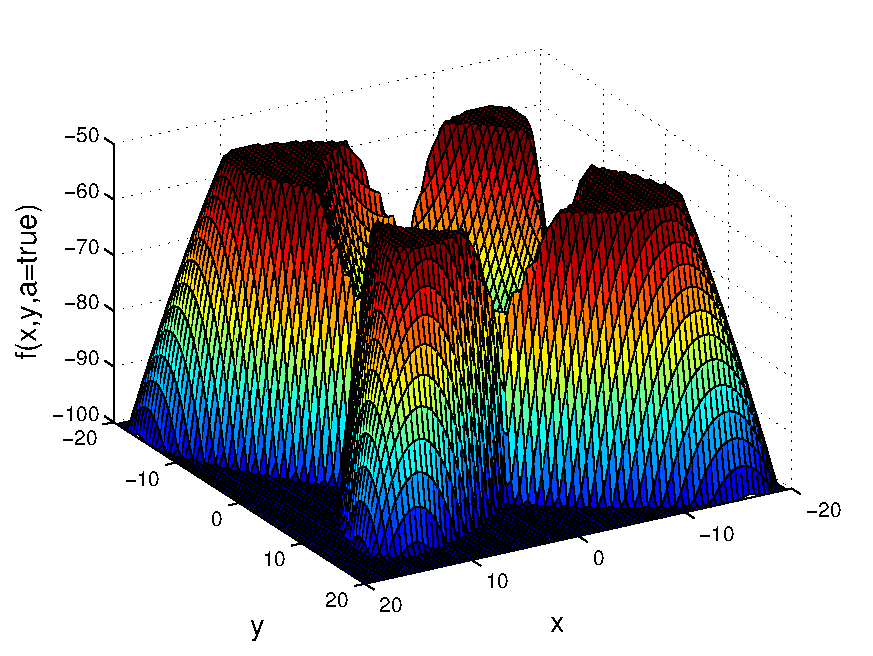
\includegraphics[width=1.0\linewidth]{images/quad2.pdf}
%%        \caption{$f(x, y, a=\mathit{true})$}
%    \end{subfigure}
%            \hspace{-5mm}
%    \begin{subfigure}[b]{0.24\textwidth}
%
%        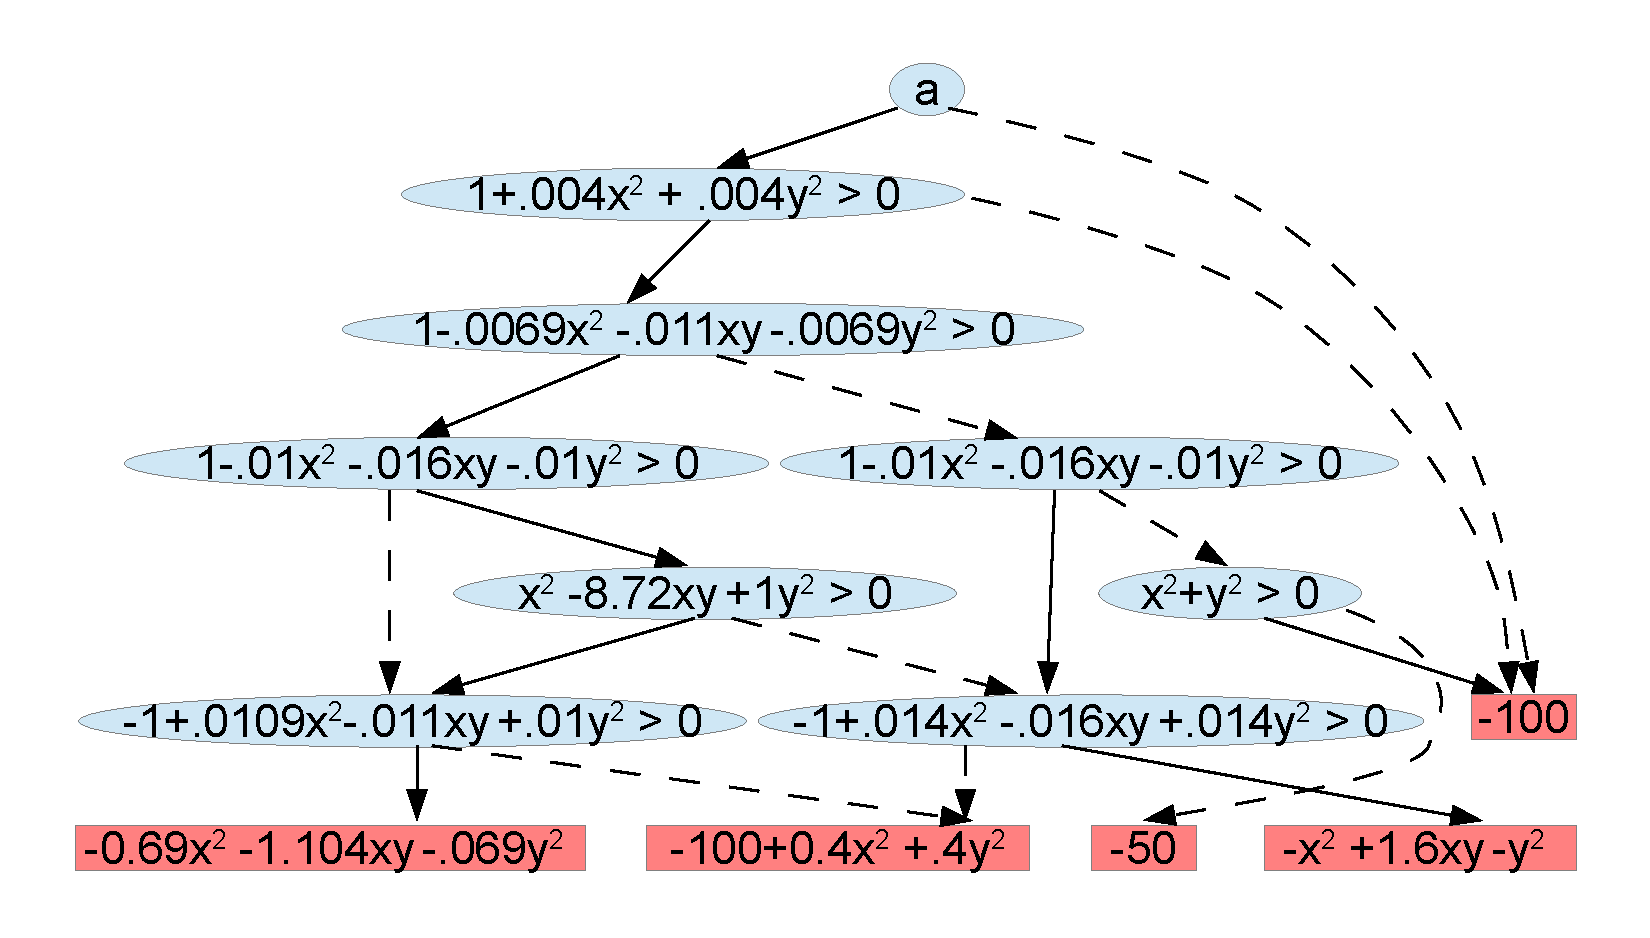
\includegraphics[width=1.3\linewidth, height=1.0\linewidth]{images/quad2_xadd5.pdf}
%%        \caption{XADD representation}        
%    \end{subfigure}    
%    \caption{(left) A plot of a function $f(x, y, a=\mathit{true})$ for continuous variables $x$ and $y$ and boolean variable $a$; and (right) its XADD representation.}
%    \label{fig:xadd}
%\end{figure}


\subsection{SDP for Parameterized Hybrid MDPs}

Value iteration (VI)~\parencite{Bellman_PU_1957} can be modified to solve continuous state and parameter PHMDPs in terms of the following case operations:
%To calculate the exact solution to PHMDPs we begin by replacing all functions and operations in Equations~\eqref{eq:vi_qfunc} and~\eqref{eq:vi_vfunc} by their case statement equivalents: 
%That is, we exchange operations such as {\footnotesize$+$}, {\footnotesize$\times$} and {\footnotesize$\max$}, by their symbolic equivalents, {\footnotesize$\oplus$}, {\footnotesize$\otimes$} and $\casemax$, respectively, and express {\footnotesize $\Reward(\vec{d}, \vec{x}, a; \vec{\theta})$},  {\footnotesize $\ProbArg{\vec{d}', \vec{x}' | \vec{d}, \vec{x}, a, \vec{\theta}}$}, {\footnotesize $V^0(\vec{d}, \vec{x}; \vec{\theta})$} as case statements. 
%The optimal solution to PHMDPs can now be described by the following recursive SDP equations:
{\footnotesize 
    \abovedisplayskip=0pt
    \belowdisplayskip=0pt
    \begin{align}
        Q^{h} \left( \vec{d}, \vec{x}, a; \vec{\theta} \right) = \Reward \left( \vec{d}, \vec{x}, a; \vec{\theta} \right) \oplus \gamma \, \cdot &  \nonumber \\ 
        \bigoplus_{\vec{d}'} \int_{\vec{x}'} \ProbArg{ \left. \vec{d}', \vec{x}' \middle| \vec{d}, \vec{x}, a; \vec{\theta} \right.} \otimes V^{h-1} \left( \vec{d}', \vec{x}'; \vec{\theta} \right) & \, d\vec{x}'  \label{eq:vi_sdp_qfunc} \\
        V^{h}\left( \vec{d}, \vec{x}; \vec{\theta} \right) = \casemax_{a \in \mathcal{A}} \left\{ Q^{h} \left( \vec{d}, \vec{x}, a; \vec{\theta} \right) \right\} & \label{eq:vi_sdp_vfunc}
    \end{align}
}%

{\footnotesize $\ProbArg{\left. \vec{d}', \vec{x}' \middle| \vec{d}, \vec{x}, a; \vec{\theta} \right.}$ } is specified in Equation~\eqref{eq:hmdp_tfunc}. We note that all parameters {\footnotesize $\theta_i$} that are free variables 
are encoded as {\footnotesize $\delta\left[\left(\theta_i' - \theta_i\right)\right]$}, indicating that they are stationary and hence do not change during the backup operation. Continuous state parameters {\footnotesize $ \vec{x} $} are handled in a similar fashion. All operations including action maximization will automatically condition the value on these parameters, yielding the parameterized value function in Equation~\eqref{eq:vi_sdp_vfunc}.

In the case of discrete {\footnotesize \Action} it can be proved that all of the SDP operations used in Equations~\eqref{eq:vi_sdp_qfunc} and~\eqref{eq:vi_sdp_vfunc} are closed form for NPWN functions~\parencite{Sanner_UAI_2011}. In the case of continuous {\footnotesize \Action} all of the operations are closed form for only LPWC or LPWL functions~\parencite{Zamani_AAAI_2012}.

%It can be proved that all of the SDP operations used in Equations~\eqref{eq:vi_qfunc} and~\eqref{eq:vi_vfunc} are closed form for LPWC or LPWL functions~\parencite{Sanner_UAI_2011,Zamani_AAAI_2012}. Given a LPWL {\footnotesize $V^{0}(\vec{d}, \vec{x}; \vec{\theta})$} and that SDP operations are closed form, the resulting {\footnotesize $V^{1}(\vec{d}, \vec{x}; \vec{\theta})$} is also LPWL. Therefore, by induction is {\footnotesize $V^{h+1}(\vec{d}, \vec{x}; \vec{\theta})$} LPWL for all horizons {\footnotesize $ \Horizon $}. 

\subsubsection{Inverse Learning for Multi-objective PHMDPs}

A possible formulation for the inverse learning problem for multi-objective MDPs is to 
%The inverse learning problem for multi-objective MDPs, whereby observed behavior is used to infer multi-objective weights that explain the observed behavior, has many possible formulations. One possible formulation is to 
constrain the Q-values corresponding to the observed behavior and maximize the weight {\footnotesize $ w $} that most explains the observed behavior: 
\begin{align}
    \max_w Q^{h} \left(w, \vec{d}, x, a_1; \vec{\theta}^d \right) \ominus Q^{h} \left(w, \vec{d}, x, a_2; \vec{\theta}^d \right)
\end{align}
where {\footnotesize $ x $} can either be fixed or a region specified in the constraints. The PHMDP framework permits any variant of the inverse learning problem for multi-objective MDPs.

PHMDPs with multi-objective {\footnotesize $\Reward$} and linear scalarization functions can be solved exactly and in closed-form by restricting the {\footnotesize $\Reward$} to LPWC functions and {\footnotesize $\Transition$} to LPWL functions. 
%Given a LPWL {\footnotesize $V^{0}(\vec{d}, \vec{x}; \vec{\theta})$} and SDP operations that are closed form, the resulting {\footnotesize $V^{1}(\vec{d}, \vec{x}; \vec{\theta})$} is also LPWL. Therefore, by induction {\footnotesize $V^{h+1}(\vec{d}, \vec{x}; \vec{\theta})$} is LPWL for all horizons {\footnotesize $ h \in \Horizon $}. 
Multi-objective PHMDPs with a nonlinear scalarization function and NPWN {\footnotesize $\Reward$} and {\footnotesize $\Transition$} functions lead to NPWN solutions, which are exact and closed-form~\parencite{Sanner_UAI_2011}.

\subsubsection{Sensitivity Analysis for PHMDPs}

%Sensitivity analysis for PHMDPs can be conducted exactly and in closed-form by firstly imposing the same restrictions on the {\footnotesize $\Reward$} and {\footnotesize $\Transition$} as the previous section and then differentiating the resulting value function with respect to the parameter {\footnotesize $\vec{\theta}$} i.e. {\footnotesize $\bigtriangledown_{\vec{\theta}} V^{h}\left(\vec{d}, \vec{x}; \vec{\theta}\right)$ }.

Sensitivity analysis for PHMDPs can be analysed exactly and in closed-form via SDP by first calculating Equation~\eqref{eq:vi_sdp_vfunc} and then taking symbolic derivatives, up to any order, with respect to the parameter {\footnotesize $\vec{\theta}^{d}$}.

% i.e. {\footnotesize $\bigtriangledown_{\vec{\theta}^{d}} V^{h}\left(\vec{d}, \vec{x}; \vec{\theta}^{d}\right)$}.

\subsubsection{Nonlinear Parameterized Policy Optimization Methods for PHMDPs}

Parameterized policies {\footnotesize $ \pi(\vec{\theta}^{d}) $}, where {\footnotesize $\vec{\theta}^{d}$} may be nonlinear, for PHMDPs can be analyzed exactly and in closed-form via SDP by substituting {\footnotesize $ \pi(\vec{\theta}^{d}) $} in for {\footnotesize  $ a $} in Equation~\eqref{eq:vi_sdp_qfunc}. This precludes the need for action maximization in Equation~\eqref{eq:vi_sdp_vfunc}. Because this function is parametric, it is possible to take symbolic derivatives up to any order i.e. {\footnotesize $\bigtriangledown_{\vec{\theta}^{d}} Q^{h}(\vec{d}, \vec{x}, a; \vec{\theta}^{d})$ } and apply non-convex optimization tools
%, such as dReal or dOp~\parencite{Gao2013}, 
that exploit parametric knowledge of the function. 
%Symbolic derivatives avoid the stochasticity issues associated with traditional policy gradient methods.

%In the next section we demonstrate how PHMDPs can be combined with SDP and state-of-the-art nonlinear optimization techniques to solve hard nonlinear sequential decision problems that were previously impossible.
    \section{Results}
\label{sec:results}

In this section we demonstrate the utility of our novel framework on three hitherto uninvestigated questions: (i) an exact functional representation of the multi-objective trade-offs in a multi-objective navigation domain; (ii) exact sensitivity analysis of public health policies in epidemic models over the full range of infection rate parameters; and (iii) non-convex optimization of policy parameters applied to finance problems previously impossible with sample-based policy gradient techniques.

\subsection{Multi-objective Navigation}
\label{sec:results_navigation}

In this domain we consider an autonomous vehicle moving along one dimension, e.g. along the real number line. At each stage the vehicle must trade-off between moving into a potentially higher reward region and incurring a cost associated with movement. The domain is specified as follows:
\begin{itemize}
    \item {\footnotesize $ \State = \left\langle loc \right\rangle$}, where $ loc $ is the location of the vehicle.
    \item {\footnotesize $ \Action \in \left\lbrace -5.0, 0.0, 5.0 \right\rbrace $} is the amount by which vehicle moves relative to its current location.
    \item {\footnotesize $ \Transition\left( loc' | loc, a \right) = \delta \left[ loc' - (loc + a) \right] $}
    \item {\footnotesize $ \Reward\left(\vec{w}, loc, a, \mathtt{threshold} \right) = w_1 \cdot \Reward_{\mathtt{location}} + w_2 \cdot \Reward_{\mathtt{movement}} $} where, \\
    {\footnotesize 
        \abovedisplayskip=10pt
        \belowdisplayskip=0pt
        \renewcommand{\arraystretch}{1.5}
        \begin{tabular}{ll}    
            $ \Reward_{\mathtt{location}}(loc', a, \mathtt{threshold}) = $ &  $ $ \\
                \qquad $ \begin{cases}
                (loc' \geq \mathtt{threshold}) : & loc' \\
                \text{otherwise} : & 0.0 \\
                \end{cases} $ & $ $\\
            $ \Reward_{\mathtt{movement}}(loc', a) = -cost_{\mathtt{movement}} $ & $ $ \\                        
        \end{tabular}
    }    
\end{itemize} 

In Figure~\ref{fig:vehicle1d} we present the optimal {\footnotesize$ \Horizon = 10 $} value function for the multi-objective navigation domain with {\footnotesize $ \mathtt{threshold} = 10.0 $} and {\footnotesize$ cost_{\mathtt{movement}} = -1.0 $}. The value function shows that when the location of the vehicle is below the {\footnotesize $ \mathtt{threshold} $}, the actions of the vehicle depends on the value of {\footnotesize $ w_2 $}; large values of {\footnotesize $ w_2 $} leads to the vehicle staying in its current location, whereas at smaller values of {\footnotesize $ w_2 $}, the vehicle is likely to move towards the goal region and incur the movement cost.
%------------------------------------------------------------------------------
% Figure
\begin{figure}[h!]
    \centering
    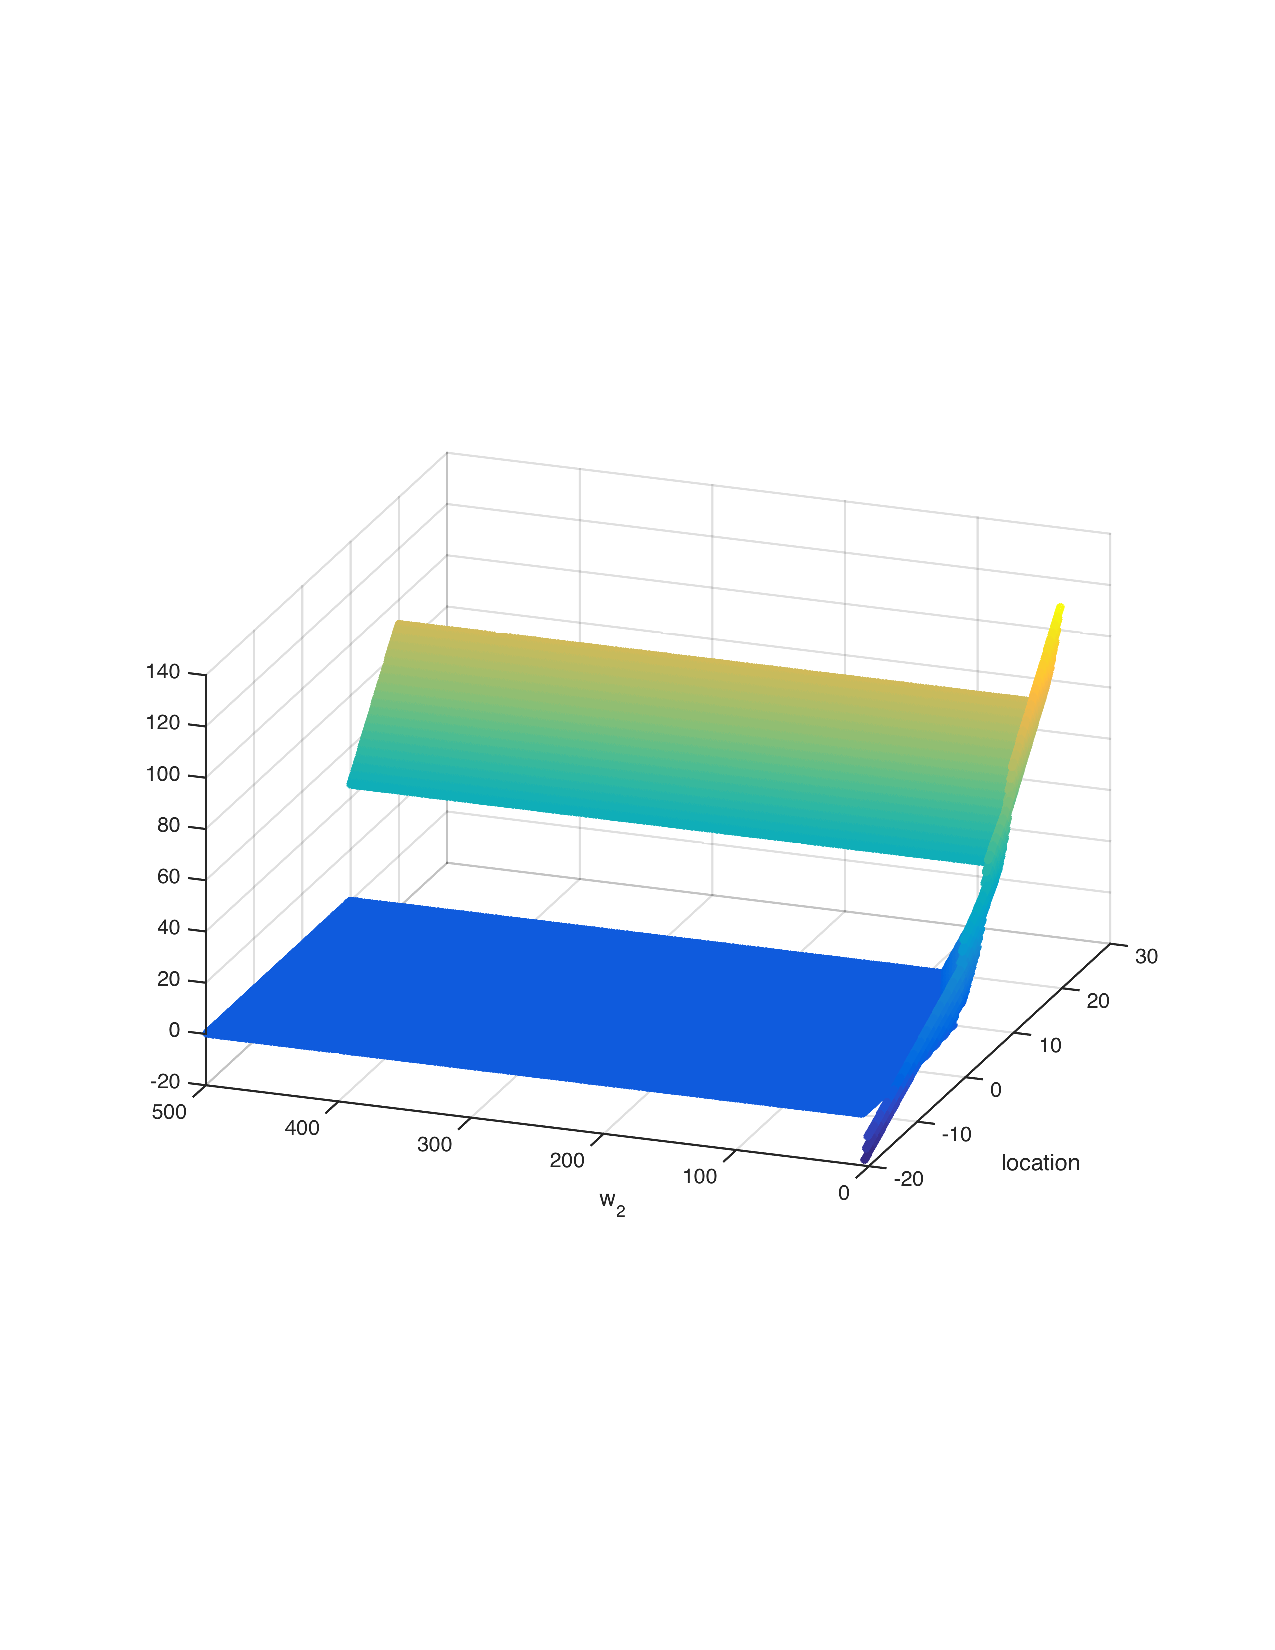
\includegraphics[width=0.8\linewidth, height=0.6\linewidth]{images/robot1d}
    \caption{The optimal value function for the multiobjective navigation domain.}
    \label{fig:vehicle1d}            
\end{figure}
%------------------------------------------------------------------------------

\subsection{Influenza Public Health Policy}
\label{sec:results_influenza}

Influenza viruses continuously challenge both human and avian posts with new variants causing complex epidemics. Compartmental models are widely used within epidemiology to investigate the spread of infection diseases. In this domain we investigate the sensitivity of two different Influenza models to an infection rate parameter. 

\subsubsection{S-I Model}
\label{sec:results_influenza_sd}

A simple epidemiological model is the two compartment S-I, model where {\footnotesize $ s_t $} refers to the number of susceptibles and {\footnotesize $ i_t $} to the number of infected. At each time step the population in each of the three populations is updated according to the following equations:
{\footnotesize
\begin{align*}
    s_{t + 1} &= - s_t \cdot ( \eta + a ) \\
    i_{t+1} &= \eta \cdot s_t 
\end{align*}
}
where {\footnotesize $ \eta \in [0, 1]$} is the rate of infection and {\footnotesize $ a_t \in \left\lbrace 0, \ldots, 1.0\right\rbrace $} is the proportion of susceptibles {\footnotesize $ s_t $} to be vaccinated. The S-I model can be formulated as an parameterized MDP as follows:
\begin{itemize}
    \item {\footnotesize $ \State = \left\langle s, i \right\rangle$ }, where $ s $ and $ i $ are as defined above
    \item {\footnotesize $ \Action \in \left\lbrace 0, 0.25, 0.50, 1.0 \right\rbrace $} is the proportion of $ s $ to vaccinate
    \item The transition function {\footnotesize \Transition} for each state variable in {\footnotesize \State} is given by:    \\
    {\footnotesize 
        \abovedisplayskip=5pt
        \belowdisplayskip=0pt
        \renewcommand{\arraystretch}{1.5}
        \begin{tabular}{ll}
            $ \Transition\left( s' | s, i, a \right) =$ & $ \delta \left[ s' - (- s \cdot (\eta + a)) \right] $ \\
            $ \Transition\left( i' | s, i, a \right) =$ & $ \delta \left[ i' - (\eta \cdot s) \right] $ \\
        \end{tabular}
    }%
    \item {\footnotesize $ \Reward\left(\vec{w}, cost_{\mathtt{inf}}, cost_{\mathtt{vaccine}}, s, i, a \right) = w_1 \cdot \Reward_{\mathtt{inf}} + w_2 \cdot \Reward_{\mathtt{vaccine}}$} where, \\
%    {\footnotesize $ cost_{\mathtt{inf}} $} is the incident cost of infection and {\footnotesize $ cost_{\mathtt{vaccine}} $} is the unit cost of vaccination \\
    {\footnotesize 
        \abovedisplayskip=10pt
        \belowdisplayskip=0pt
        \renewcommand{\arraystretch}{1.5}
        \begin{tabular}{ll}    
            $ \Reward_{\mathtt{inf}}(s', i', a, cost_{\mathtt{inf}}) = $ &  $ $ \\
                \qquad $ \begin{cases}
                (i \geq 0) : & cost_{\mathtt{death}} \cdot i \\
                \text{otherwise} : & 0 \\
                \end{cases} $ & $ $ \\
            $ \Reward_{\mathtt{vaccine}}(s', i', a, cost_{\mathtt{vaccine}}) = $ &  $ $ \\
                \qquad $ \begin{cases}
                (s \geq 0) : & cost_{\mathtt{vaccine}} \cdot s \cdot a \\
                \text{otherwise} : & 0 \\
                \end{cases} $ & $ $ \\
        \end{tabular}
    }    
\end{itemize} 

Figure~\ref{fig:influenza_sd} displays the sensitivity of the optimal {\footnotesize$ \Horizon = 4 $} value function for the S-I model to infection rate parameter {\footnotesize $ \eta \in \left\lbrace 0, 0.02 \right\rbrace$}. The parameters of the models were set to {\footnotesize $cost_{\mathtt{inf}} = 95.0$} and {\footnotesize$cost_{\mathtt{vaccine}} = 33.0$}. From the Figure it is clear that as the number of susceptibles {\footnotesize $ s $} increases, an increase in the infection rate parameter {\footnotesize $ \eta $}, leads to a deleterious outcome for the population.
%------------------------------------------------------------------------------
% Figure
\begin{figure}[h!]
    \centering
    \begin{subfigure}[b]{0.4\textwidth}    
        %        \centering
        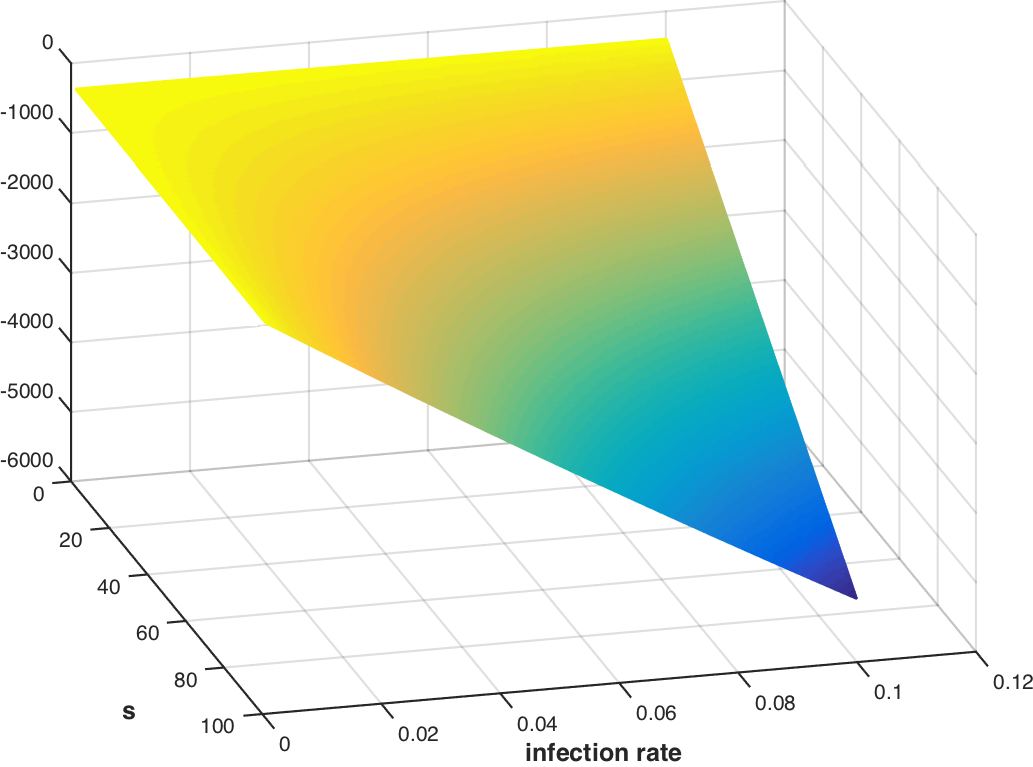
\includegraphics[width=0.8\linewidth, height=0.6\linewidth]{images/sd_infection_s}
        \caption{Optimal Influenza Epidemiology value under the S-D specification.}
        \label{fig:influenza_sd_value_function}
        \vspace{1em}
    \end{subfigure}
    
    \begin{subfigure}[b]{0.4\textwidth}    
        %        \centering
    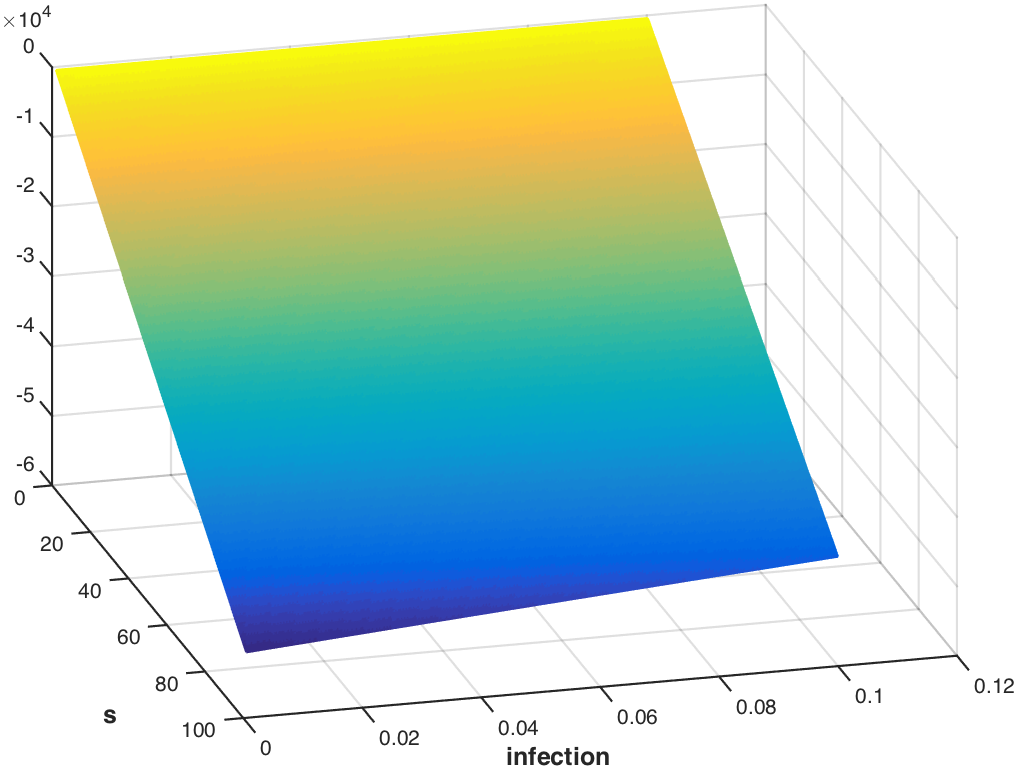
\includegraphics[width=0.8\linewidth, height=0.6\linewidth]{images/sd_infection_sensitivity}
    \caption{Sensitivity.}
    \label{fig:influenza_sd_sensitivity}
    \end{subfigure}  
    \caption{The optimal value function for the S-D model.}
    \label{fig:influenza_sd}    
\end{figure}
%------------------------------------------------------------------------------

\subsubsection{S-I-R-S Model}
\label{sec:results_influenza_sirs}

A more complex epidemiological model is the three compartment S-I-R-S, model where {\footnotesize $ s_t $} refers to the number of susceptibles, {\footnotesize $ i_t $} to number of infected and {\footnotesize $ r_t $} to the recovered. At each time step the population in each of the three populations is updated according to the following equations:
{\footnotesize
\begin{align*}
    s_{t + 1} &= -\eta \cdot s_t \cdot i_t + \lambda \cdot r_t - a_t \cdot s_t \\
    i_{t + 1} &= \eta \cdot s_t \cdot i_t - \beta \cdot i_t \\
    r_{t+1} &= \beta \cdot i_t - \lambda \cdot r_t 
    %    d_{t+1} &= e \cdot i_t 
\end{align*}
}
where {\footnotesize $ \eta \in [0, 1]$} is the rate of infection, {\footnotesize $ \beta \in [0, 1]$} is the rate of recovery and {\footnotesize $ \lambda \in [0, 1]$} is the rate of susceptibility, and {\footnotesize $ a_t \in \left\lbrace 0, \ldots, 1.0\right\rbrace $} is the proportion of susceptibles {\footnotesize $ s_t $} to be vaccinated. The S-I-R-S model can be formulated as an parameterized MDP as follows:
\begin{itemize}
    \item {\footnotesize $ \State = \left\langle s, i, r \right\rangle$ }, where $ s $, $ i $, and $ r $ are as defined above
    \item {\footnotesize $ \Action \in \left\lbrace 0, 0.25, 0.50, 1.0 \right\rbrace $} is the proportion of $ s $ to vaccinate
    \item The transition function {\footnotesize \Transition} for each state variable in {\footnotesize \State} is given by:    \\
    {\footnotesize 
        \abovedisplayskip=5pt
        \belowdisplayskip=0pt
        \renewcommand{\arraystretch}{1.5}
        \begin{tabular}{ll}
            $ \Transition\left( s' | s, i, r, a \right) =$ & $ \delta \left[ s' - (- \eta \cdot s \cdot i + \lambda \cdot r -a \cdot s) \right] $ \\
            $ \Transition\left( i' | s, i, r, a \right) =$ & $ \delta \left[ i' - (\eta \cdot s \cdot i - \beta \cdot i) \right] $ \\
            $ \Transition\left( r' | s, i, r, a \right) =$ & $ \delta \left[ r' - (\beta \cdot i - \lambda \cdot r) \right] $ \\            
        \end{tabular}
    }%
    \item {\footnotesize $ \Reward\left(\vec{w}, cost_{\mathtt{inf}}, cost_{\mathtt{vaccine}}, s, i, r, a \right) = w_1 \cdot \Reward_{\mathtt{inf}} + w_2 \cdot \Reward_{\mathtt{vaccine}}$} where, \\
%    {\footnotesize $ cost_{\mathtt{inf}} $} is the incident cost of infection and {\footnotesize $ cost_{\mathtt{vaccine}} $} is the unit cost of vaccination \\
    {\footnotesize 
        \abovedisplayskip=10pt
        \belowdisplayskip=0pt
        \renewcommand{\arraystretch}{1.5}
        \begin{tabular}{ll}    
            $ \Reward_{\mathtt{inf}}(s', i', r', a, cost_{\mathtt{death}}) = $ &  $ $ \\
            \qquad $ \begin{cases}
            (i \geq 0) : & cost_{\mathtt{death}} \cdot i \\
            \text{otherwise} : & 0 \\
            \end{cases} $ & $ $ \\
            $ \Reward_{\mathtt{vaccine}}(s', i', a, cost_{\mathtt{vaccine}}) = $ &  $ $ \\
            \qquad $ \begin{cases}
            (s \geq 0) : & cost_{\mathtt{vaccine}} \cdot s \cdot a \\
            \text{otherwise} : & 0 \\
            \end{cases} $ & $ $ \\
        \end{tabular}
    }    
%    \item {\footnotesize $ \Reward\left(\vec{w}, cost_{\mathtt{inf}}, s, i, r, a \right) = w_1 \cdot -cost_{\mathtt{inf}} \cdot i + w_2 \cdot -cost_{\mathtt{vaccine}} \cdot a $}, where {\footnotesize $ cost_{\mathtt{inf}} $} is the incident cost of infection and {\footnotesize $ cost_{\mathtt{vaccine}} $} is the unit cost of vaccination \\
\end{itemize} 

Figure~\ref{fig:influenza_sirs} displays the sensitivity of the optimal {\footnotesize$ \Horizon = 4 $} value function for the S-I-R-S model to infection rate parameter {\footnotesize $ \eta \in \left\lbrace 0, 0.02 \right\rbrace$}. The parameters of the models were set to {\footnotesize$ \beta = 0.27, \lambda = 0.23, cost_{\mathtt{inf}} = 95.0$} and {\footnotesize$cost_{\mathtt{vaccine}} = 33.0$}. From the Figure it is clear that the deleterious affect of an increasing {\footnotesize $ \eta $} is counteracted by the amount of individuals becoming susceptible due to the rate of susceptibility {\footnotesize $ \lambda $}.
%------------------------------------------------------------------------------
% Figure
\begin{figure}[t!]
    \centering
    \begin{subfigure}[b]{0.4\textwidth}    
        %        \centering
        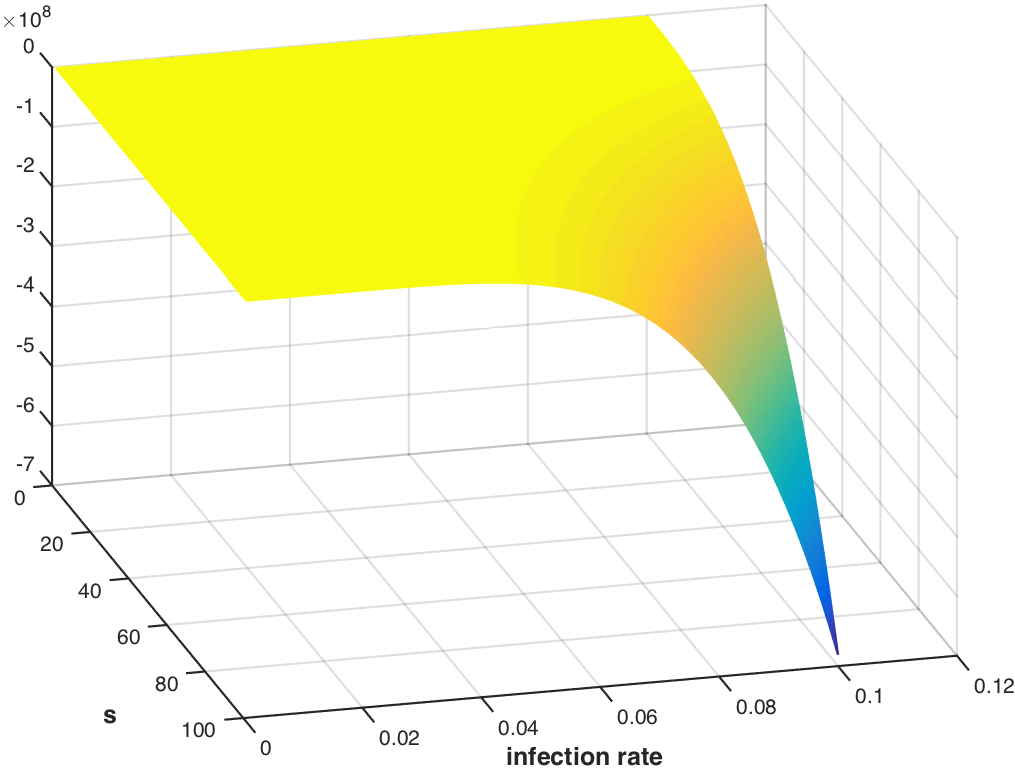
\includegraphics[width=0.8\linewidth, height=0.6\linewidth]{images/sir_infection_s}
        \caption{Optimal Influenza Epidemiology value under the S-I-R-S specification.}
        \label{fig:influenza_sirs_value_function}
        \vspace{1em}
    \end{subfigure}
    
    \begin{subfigure}[b]{0.4\textwidth}    
        %        \centering
        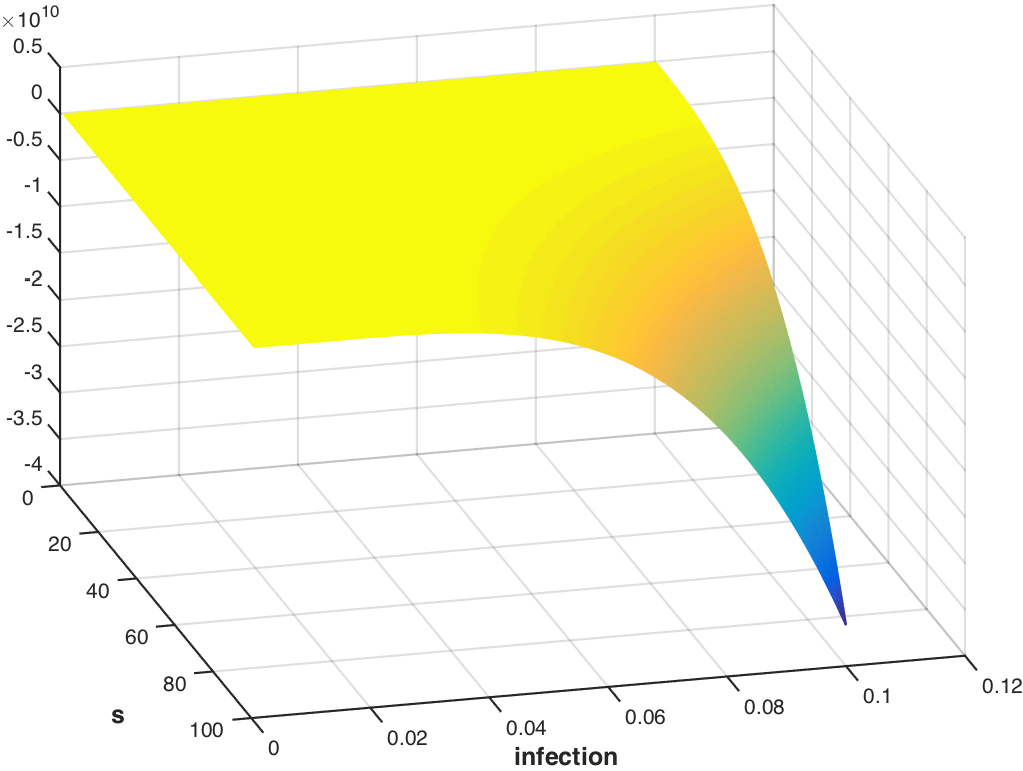
\includegraphics[width=0.8\linewidth, height=0.6\linewidth]{images/sir_infection_sensitivity}
        \caption{Sensitivity.}
        \label{fig:influenza_sirs_sensitivity}
    \end{subfigure}  
    \caption{The optimal value function for the S-I-R-S model.}
    \label{fig:influenza_sirs}      
\end{figure}
%------------------------------------------------------------------------------

\subsection{Optimal Execution}
\label{sec:results_oe}

Institutional investors often need to acquire or liquidate a number of shares within a given period of time. Indirect transaction costs are an important consideration for institutional investors who often want to transact a number of shares that exceeds the available liquidity i.e. there may not be counterparty or counterparties that wish to take the other side of the trade at the same volume. There is a clear trade-off between the market impact of transacting immediately and the volatility of slow execution. 

In this domain we use a price impact model inspired by Bertsimas and Lo~\parencite{Bertsimas_JFM_1998} to investigate the optimisation of parameters within two static policies: (1) constant liquidation; and (2) fractional liquidation. The common components of the optimal execution domain for each type of static policy can be defined as:
\begin{itemize}
    \item {\footnotesize $ \State = \left\langle price, inv \right\rangle$}, where $ price $ is the price of the asset and $ inv $ is the inventory remaining
    \item  {\footnotesize $ \Transition\left( price' | price, inv, a \right) = \delta \left[ price' - (price + \kappa + \sigma \cdot \epsilon) \right] $}
\end{itemize}

\subsubsection{Constant Liquidation Policy}
\label{sec:results_oe_constant}

With a constant liquidation policy the investor chooses to sell a constant number of assets at each time period. This specific scenario is defined by the following:
\begin{itemize}
    \item {\footnotesize 
         \begin{tabular}{ll}
            $ \Transition\left( inv' | price, inv, a \right) = $ & $ $ \\
            $ \qquad \delta \left[ inv' - \begin{cases}
            inv \geq a : & inv - a \\
            \text{otherwise} : & inv \\
            \end{cases} \right] $ & $ $\\
        \end{tabular}
    }%
    \item {\footnotesize $ \Reward\left(price, price_0, inv, a \right) =
        \begin{cases}
            (inv \geq a) : & a \cdot price - a \cdot price_0 \\
            \text{otherwise} : & 0 \\
        \end{cases} $}
    \item {\footnotesize $ \Action \in \left\lbrace 0, \ldots, inv \right\rbrace $} is the number of the remaining inventory to sell    
\end{itemize}

\subsubsection{Fractional Liquidation Policy}
\label{sec:results_or_fractional}

With a fractional liquidation policy the investor chooses to sell a constant proportion of assets at each time period. This specific scenario is defined by the following:
\begin{itemize}
    \item {\footnotesize $\Transition\left( inv' | price, inv, n \right) = \delta \left[ inv' - (inv - inv \cdot a) \right] $}
    \item {\footnotesize $ \Reward\left(price, price_0, inv, a \right) =
        \begin{cases}
        (inv \geq a) : & a \cdot inv \cdot price - inv \cdot price_0 \\
        \text{otherwise} : & 0 \\
        \end{cases} $} 
    \item {\footnotesize $ \Action \in \left\lbrace 0, 0.25, 0.50, 1.0 \right\rbrace $} is the proportion of the remaining inventory to sell    
\end{itemize}

The investor aims to minimise implementation shortfall, which is defined as the difference between the theoretical benchmark price and the actual price received is the implementation shortfall~\parencite{Perold_JPM_1988}.

Figure~\ref{fig:opt_execution} displays the sensitivity of the optimal {\footnotesize$ \Horizon = 5 $} value function for the optimal execution model under both static policies. The parameters of the models were set to {\footnotesize$ \kappa = 0.0.0165, price_0 = 10.0, price = 20.0$} and {\footnotesize$inv = 200.0$}. 
%------------------------------------------------------------------------------
% Figure
\begin{figure}[t!]
    \centering
    \begin{subfigure}[b]{0.4\textwidth}    
%        \centering
        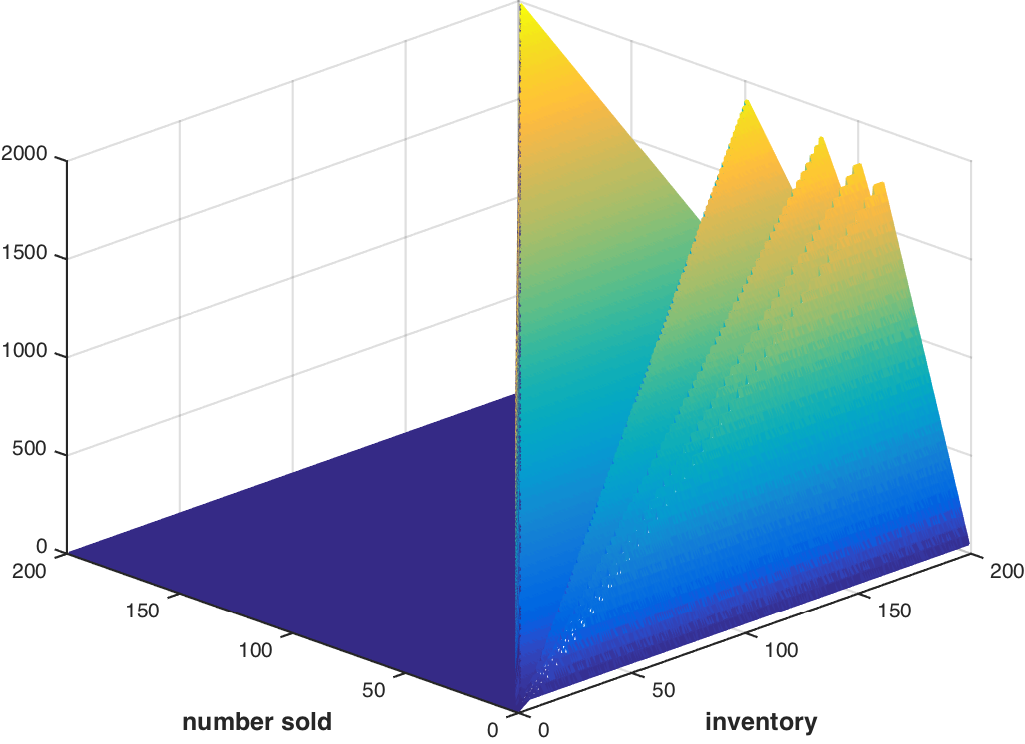
\includegraphics[width=\linewidth, height=0.6\linewidth]{images/opt_execution_budget}
        \caption{Constant liquidation.}
        \label{fig:opt_execution_w1}
        \vspace{1em}
    \end{subfigure}
    
    \begin{subfigure}[b]{0.4\textwidth}    
%        \centering
        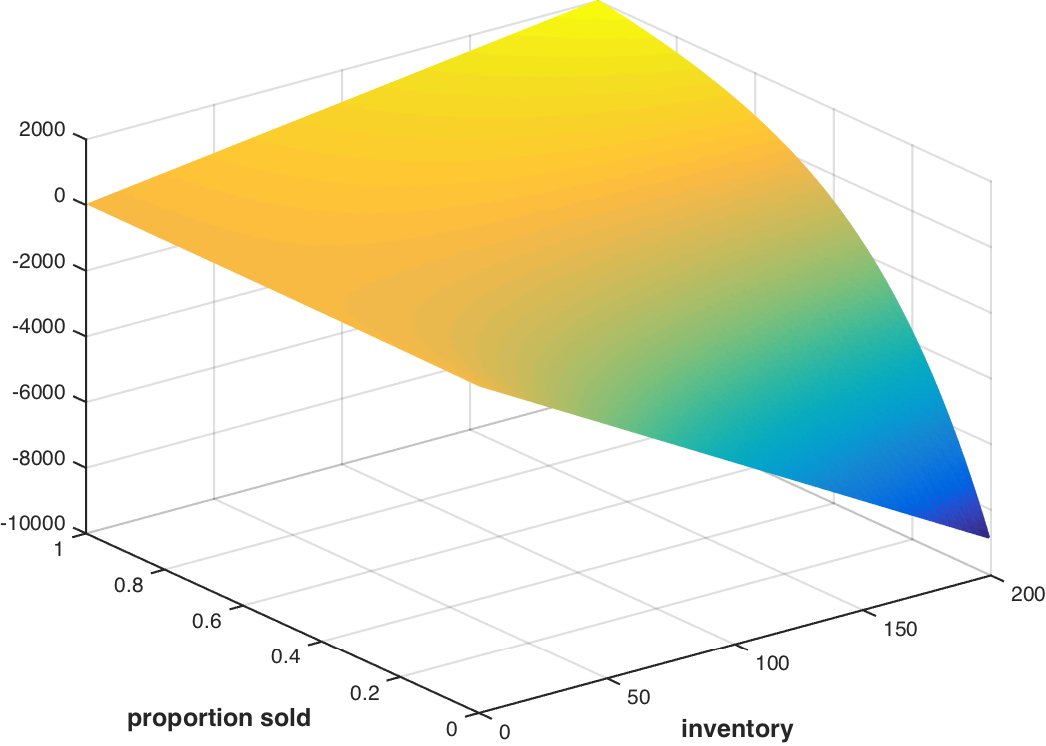
\includegraphics[width=\linewidth, height=0.6\linewidth]{images/opt_execution_fraction}
        \caption{Fractional liquidation.}
        \label{fig:opt_execution_w2}
    \end{subfigure}  
    \caption{The optimal execution value function under different policies.}
    \label{fig:opt_execution}
\end{figure}
%------------------------------------------------------------------------------
    \section{Conclusions}
\label{sec:conclusion}

In this paper we introduced Parameterized Hybrid MDPs as a unifying framework, which enables the inverse learning of parameters of multi-objective rewards, the examination of parameter sensitivity and the non-convex optimization of continuous policy parameters. We also presented a novel algorithm to solve PHMDPs by utilizing a parametric extension of symbolic dynamic programming and state-of-the-art non-convex optimizers. We demonstrated the utility and scalability of our framework by calculating the first known exact solutions to the inverse learning of parameters for multi-objective navigation, non-convex optimization of vaccination policies and sensitivity analysis of trading models.

There are a number of avenues for future research. Firstly, it is important to examine more general representations of the reward and transition functions while still guaranteeing exact solutions. Another direction of research lies within improving the scalability of the algorithm by either extending techniques for Algebraic Decision Diagrams~\cite{Bahar_JoFMiSD_1993} from APRICODD~\cite{St-Aubin_NIPS_2000} under the current restrictions on the reward and transition functions or bounded error compression for XADDs~\cite{Vianna_UAI_2013} for more expressive representations. The advances made within this paper open up a number of potential novel research paths, which may be used to progress multi-objective analyses, sensitivity analyses and nonlinear parameterized policy optimization for difficult nonlinear sequential decision making problems.


%--------------------------------------------------------------------------------------------------
% Bibliography
%--------------------------------------------------------------------------------------------------
\newpage
{\small
\printbibliography
}
\end{document}